\section{Modelo de esparcimiento coherente}

La solución de Mie en conjunto con la corrección por tamaño a la función dieléctrica para algún material, permite estudiar la respuesta electromagnética de una NP esférica individual y calcular las frecuencias de resonancia de los plasmones localizados de superficie (Localized Surface Plasmons Resonances, LSPRs), empleados en la espectroscopía \cite{novotny2006principles}, el sensado \cite{jain2008noble} y la litografía \cite{stockman2011nanoplasmonics}\index{Plasmón!de Superficie Localizado (LSP)!Resonancia de (LSPR)}. Sin embargo, no siempre es posible emplear la respuesta EM de una partícula individual para la descripción de un sistema compuesto de muchas partículas ---como una monocapa de NPs---, por lo que se han empleado diversos enfoques entre los que se encuentran la aproximación cuasiestática y las teorías de esparcimiento múltiple \cite{reyes2018analytical,pena-gomar2006coherent,barrera2003coherent,garcia2012multiple}\index{Esparcimiento!Múltiple (MS)}. En el caso límite de partícula pequeña, donde el parámetro de tamaño $x=ka\ll 1$, con $k$ el número de onda dentro de la matriz donde se encuentran inmersas las NPs, suponiéndolas esféricas con un radio $a$, es posible emplear  la aproximación cuasiestática, que considera que sólo la excitación dipolar contribuye al campo total \cite{reyes2018analytical}. En partícular,  bajo la aproximación cuasiestática, es posible desarrollar una teroía de medio efectivo para calcular la reflectancia de una monocapa de NPs \cite{pena-gomar2006coherent,barrera1991optical}. Sin embargo, cuando  el parámetro de tamaño es comparable o mayor a la unidad, una teoría de esparcimiento múltiple es necesaria, debido a la excitación de multipolos de ordenes mayores \cite{pena-gomar2006coherent}. El modelo de esparcimiento coherente (Coherent Scattering Model, CSM)\index{Esparcimiento!Coherente, Modelo de (CSM)} toma en cuenta la interacción de esparcidores ante la presencia de un campo eléctrico promedio; este enfoque además incluye la contribución del esparcimiento múltiple debido a la interacción entre las NPs \cite{reyes2018analytical}.
    
    El cálculo de las expresiones para la reflectancia y la transmitancia en el formalismo del CSM considera el campo eléctrico total esparcido por una monocapa de NPs. En general, éste puede descomponerse en una componente coherente ---respuesta promedio con una dirección de propagación bien definida--- y una componente difusa ---causada por las fluctuaciones y cuya propagación se da en todas las direcciones--- \cite{tsang2000scattering}, como se muestra en la Fig. \ref{fig:CSM-Slab}, en donde un arreglo desordenado de NPs inmersas en una matriz se ilumina con una onda plana monocoromática en la dirección $\vb{k}^i$, y en donde las flechas rojas corresponden a los vectores de onda del campo eléctrico esparcido por NPs en la dirección coherente, mientras que las flechas rosas corresponden a los vectores de onda del campo eléctrico esparcido difuso. Para definir los coeficientes de amplitud de reflexión $r$ y transmisión $t$ para una arreglo desordenado de NPs inmersas en una matriz, se toma en cuenta  únicamente la componente coherente al asumir que la cantidad de energía que porta la componente difusa es mucho menor que la que porta la coherente \cite{reyes2018analytical}. Para el cálculo de $r$ y $t$, primero se calculan los coeficientes de amplitud de reflexión y transmisión de una monocapa de NPs suspendida en el espacio libre (Free Standing Monolayer, FSM), es decir, inmersa en un medio dieléctrico denominado matriz, seguido del efecto de introducir una interfaz con un medio denominado sustrato. La reflectancia del sistema sustrato-monocapa-matriz se resuelve al considerar  multiples reflexiones en la interfaz entre las superficies dadas por la interfaz sustrato-matriz y monocapa-matriz. 
 
\begin{figure}[h!]\centering
	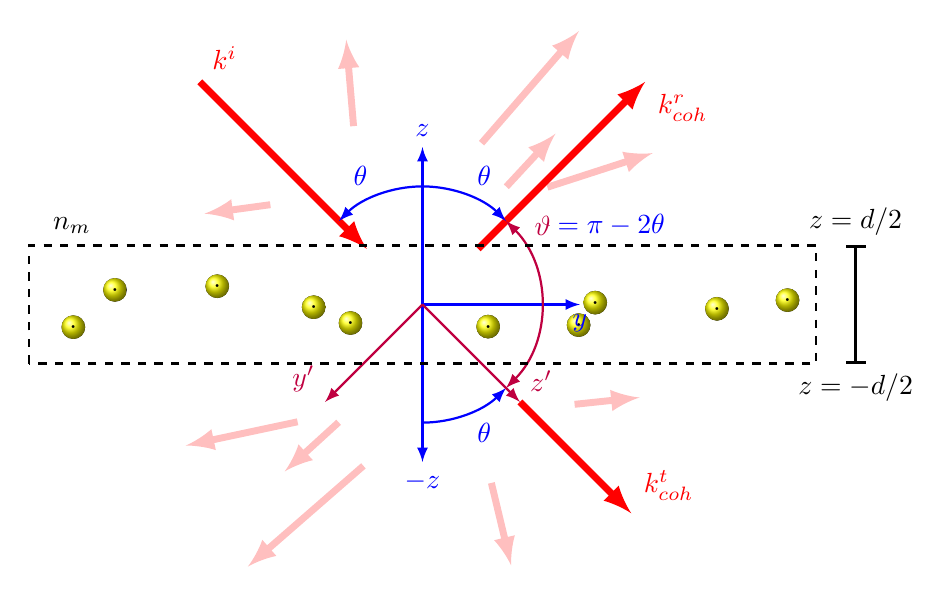
\begin{tikzpicture}[scale=1]
\def\a{.15}
\def\d{.75}
%----------------------NPs--------------
\foreach \y in {-4.5,-3.5,...,3.5,4.5}{
\fill[ball color=yellow, opacity=1] (\y+rand*.5,rand*.45) circle(\a) node[ ]{.};
}

%----------------------difussed scattered field--------------
\begin{scope}[opacity=.25, transparency group]
\foreach \s in {-1,1}{
	\draw[- latex, red, line width=2.5](0,\s*\d)++(25:\s*1.75)--(35+rand*5:\s*3.5);
	\draw[- latex, red, line width=2.5](0,\s*\d)++(35:\s*1.3)--(55+rand*5:\s*2.75);
	\draw[- latex, red, line width=2.5](0,\s*\d)++(165:\s*2)--(155+rand*5:\s*3);
	\draw[- latex, red, line width=2.5](0,\s*\d)++(120:\s*1.75)--(110+rand*5:\s*3.5);
	\draw[- latex, red, line width=2.5](0,\s*\d)++(60:\s*1.5)--(60+rand*5:\s*4);}
\end{scope}

%----------------------coherent scattered field--------------
\draw[latex -, thick, red, line width=2.5](135:1)--(135:4) node[anchor=south west]{$\vb{k}^i$};
\draw[- latex, thick, red, line width=2.5](45:1)--(45:4)node[anchor=north west]{$\vb{k}_{coh}^r$};
\draw[ - latex, thick, red, line width=2.5](-45:1.75)--(-45:3.75) node[anchor=south west]{$\vb{k}_{coh}^t$};

%----------------------Main system--------------
\draw[- latex, thick, blue] (0,0)--(90:2) node[anchor = south]{$z$};
\draw[- latex, thick, blue] (0,0)--(-90:2) node[anchor = north]{$-z$};
\draw[- latex, thick, blue] (0,0)--(0:2) node[anchor = north]{$y$};
\path (0,0)++(135/2:1.5)node[anchor=south west, blue]{$\theta$}; 
\draw[- latex, thick, blue](90:1.5)arc(90:45:1.5);
\path (0,0)++(-135/2:1.5)node[anchor=north west, blue]{$\theta$}; 
\draw[- latex, thick, blue](-90:1.5)arc(-90:-45:1.5);
\path (0,0)++(90+45/2:1.5)node[anchor=south east, blue]{$\theta$}; 
\draw[- latex, thick, blue](90:1.5)arc(90:135:1.5);

----------------------Mie system--------------
\draw[- latex, thick, purple] (0,0)--(-45:1.75) node[anchor = south west]{$z'$};
\draw[- latex, thick, purple] (0,0)--(-135:1.75) node[anchor = south east]{$y'$};
\path (0,0)++(30:1.5)node[anchor=south west, purple]{$\vartheta$}; 
\path (0,0)++(30:1.5)node[anchor=south west, blue]{$\;\;\; =  \pi - 2\theta$}; 
\draw[latex - latex, thick, purple](-45:1.5)arc(-45:45:1.5);

%----------------------thickness and slab-------------
\draw[thick, dashed] (-5,-\d) rectangle (5,\d);
%\draw[thick, dashed] (-5, 0) --  (5,0);
\draw[ |-|, thick,] (5.5,-\d) node[anchor = north]{$z=-d/2$} -- (5.5,\d) node[anchor = south]{$z=d/2$};
\node at (-4.5,1) {$\; n_m$};
\end{tikzpicture}
	\caption{Placa de grosor $d$ y volumen $V$ con $N$ partículas esféricas  idénticas, localizadas al azar e iluminadas con una onda plana monocromática con vector de onda $\vb{k}^i$. La dirección de los campos esparcidos coherentes se denotan por $\vb{k}^r_{coh}$ y $\vb{k}^t_{coh}$. Las flechas rojas sólidas representan las componentes coehrentes del campo esparcido mientras que las rosas represetan la componente difusa. }\label{fig:CSM-Slab}
	\end{figure} 
 
\subsection{Monocapa suspendida en el espacio libre}
 
Para calcular los coeficientes de amplitud de reflexión y transmisión del CSM se calcula el campo eléctrico promedio esparcido por las NPs dentro de la región del espacio, caracterizado por un índice de refracción real $n_m$, delimitada por  $-d/2<z<d/2$, una placa de grosor $d$ y volumen $V$, en donde se encuentran $N$ nanopartículas esféricas idénticas, con índice de refracción $n_p$, y distribuidas espacialmente de forma aleatoria, como se observa en la Fig. \ref{fig:CSM-Slab}. Si una onda plana $\vb{E}^i = E_0 e^{i\vb{k}^i\cdot\vb{r}}\vu{e}_i$ (por simplicidad se omite la dependecia temporal), con $\vu{e}_i$ un vector en el plano de polarización de la onda plana y $|\vb{k}^i| = k = 2\pi n_m /\lambda$, incide sobre la placa, el campo eléctrico esparcido  por las NPs dentro de la placa $\vb{E}^s$ (asumiendo una densidad $N/V$ baja), puede calcularse bajo la aproximación de esparcimiento individual (Single Scattering Approximation, SSA)\index{Esparcimiento!Individual, Aproximación de (SSA)}, en donde cada NP esparce la luz sin considerar la interacción entre el campo eléctrico esparcido por las otras NPs \cite{barrera2003coherent}. Al considerar la interacción del campo eléctrico incidente con las $N$ nanopartículas dentro de la placa, el campo eléctrico esparcido por todas las partículas tiene componentes espaciales en todas las direcciones, por lo que el campo eléctrico esparcido puede descomponerse en una componente coherente y una difusa, representadas en la Fig. \ref{fig:CSM-Slab} mediante las flechas rojas y rosas, respectivamente.


El  campo eléctrico esparcido promedio $\langle \vb{E}^s\rangle$, que corresponde a la componente coherente, se calcula al considerar el promedio espacial de los campos esparcidos por las NPs dentro de la placa al suponer que la posición de una NPs es independiente de la de las demás y que la probabilidad de encontrar el centro de una NP dentro del volumen de la placa es uniforme, por lo que la componente coherente del campo esparcido es  \cite{garcia2012multiple}\index{Esparcimiento!Individual, Aproximación de (SSA)!campo eléctrico esparcido promedio}
%
	\begin{align}
	\langle \vb{E}^s\rangle =
	\begin{dcases} 
	      \langle \vb{E}^s_{r,SSA}\rangle e^{i\vb{k}^r_{coh}\cdot\vb{r}} =
	    			i \frac{N}{V}  \frac{d E_0}{2} \frac{\sin(k_z^id)}{k_z^i d} 
				\frac{\mathbb{F}(\vu{k}^r,\vu{k}^i)\cdot \vu{e}_i}{k_z^i }	e^{i\vb{k}^r_{coh}\cdot\vb{r}},		& d/2<z \\
      \langle \vb{E}^s_{t,SSA}\rangle e^{i\vb{k}^t_{coh}\cdot\vb{r}} =
 				i\frac{N}{V} \frac{d E_0}{2}\frac{\mathbb{F}(\vu{k}^i,\vu{k}^i)\cdot \vu{e}_i}{k_z^i}		
				e^{i\vb{k}^t_{coh}\cdot\vb{r}},
							& z<-d/2
   \end{dcases}
   	\label{eq:AvErEt}
	\end{align}
%
en donde $k^i_z = k^i\cos\theta$; $\vb{k}^i$ es el vector de onda del campo eléctrico incidente $\vb{E}^i = \vb{E}_0 e^{i\vb{k}^i\cdot\vb{r}}$, polarizado en la dirección $\vu{e}_i$; $\vb{k}^r_{coh}$ es la dirección de propagación de la componente coherente reflejada; $\vb{k}^t_{coh}=\vb{k}^i$ es la dirección de propagación de la componente coherente transmitida; y $\mathbb{F}$ \index{Electromagnéticos!campos!operador de campo lejano} es el operador de esparcimiento de campo lejano [Ec. \eqref{eq:FarFieldDyadic}] que depende de la dirección de propagación de la onda plana incidente $\vb{k}^i$ y la del campo esparcido $\vb{k}^s$. El término $\mathbb{F}$ no limita la solución del campo eléctrico esparcido promedio al campo lejano, puesto que es un resultado derivado de promediar la respuesta EM \cite{gutierrez2012overview}.

En la Fig. \ref{fig:CSM-Slab} se observa que la dirección de propagación de  $\langle \vb{E}^s_{r,SSA}\rangle$ en $d/2<z$, dada por el vector de onda $\vb{k}^r_{coh}$ y la de $\langle \vb{E}^s_{t,SSA}\rangle$ en  $z<-d/2$, dada por $\vb{k}^t_{coh}$, forman un ángulo $\theta$ respecto a la dirección normal a la monocapa (sitema coordenado azul). A diferencia la componente difusa (flechas rosas), la componente coherente del campo eléctrico esparcido es distinta de cero al calcular el promedio espacial, ya que los campos eléctricos esparcidos por cada NP en la placa interfieren constructivamente en las direcciones de esparcimiento $\vu{k}^s =\vu{k}^i=\vu{k}^t_{coh}$ y $\vu{k}^s =\vu{k}^r_{coh}$ \cite{garcia2012multiple}. Puesto que las NPs dentro de la placa son esféricas e idénticas, se calcula la expresión del operador de esparcimiento $\mathbb{F}(\vu{k}^s,\vu{k}^i)$ al comparar su expresión general [Ec. \eqref{eq:FarFieldDyadic}] con la matriz de esparcimiento de Mie [Ec. \eqref{eq:MieMatrix}]\index{Mie!matriz de esparcimiento de}, por lo que el operador de esparcimiento de campo lejano es
%
	\begin{align}
	\mathbb{F}(\vu{k}^s,\vu{k}^i) = \frac{1}{-ik} 
	 \mqty(S_2(\vartheta) & 0 \\ 0 & S_1(\vartheta)),
	 \label{eq:FFDydadic-Mie}
	\end{align}
%
en donde $\vartheta$ denota el ángulo entre la dirección del campo esparcido $\vu{k}^s$ y del campo incidente $\vu{k}^i$, con $\vartheta = 0$ para $\vu{k}^s = \vu{k}^t_{coh}$ y $\vartheta = \pi-2\theta$  para $\vu{k}^s = \vu{k}^r_{coh}$, como se observa en la Fig. \ref{fig:CSM-Slab}.
	
Al sustituir la Ec. \eqref{eq:FFDydadic-Mie} en la Ec. \eqref{eq:AvErEt} y multiplicar las expresiones resultantes por $(3ka^3)/(3ka^3)$, con $a$ el radio de las NPs y $k = 2\pi n_m /\lambda$, y agrupar términos, se obtienen las siguientes expresiones 
%
	\begin{subequations}\begin{align}
		\langle \vb{E}^s_{r,SSA}\rangle & = - \frac{E_0}{\cos\theta_i} \frac32  \qty(\frac{N}{V} \frac43\pi a^3)\frac{kd}{(ka)^3}   \frac{\sin(k_z^id)}{k_z^i d}  S_j(\vartheta)\vu{e}_i =
		-\alpha  \frac{\sin(k_z^id)}{k_z^i d}   S_j(\vartheta) \vb{E}_0,
		\label{eqs:EsSSAr}\\
	\langle \vb{E}^s_{t,SSA}\rangle &=  - \frac{E_0}{\cos\theta_i} \frac32
						 \qty(\frac{N}{V}\frac43\pi a^3  ) \frac{kd}{(ka)^3}  S_j(0) \vu{e}_i  
						 = - \alpha S(0) \vb{E}_0,
		\label{eqs:EsSSAt}
	\end{align}\label{eq:EsSSA}\end{subequations}
%
donde  se emplea $j=1$ para polarización $s$ y $j=2$ para $p$ en los elementos de matriz no nulos de la matriz de esparcimiento de Mie, $S_j(\vartheta)$, y donde se define $S(0) \equiv S_1(0)=S_2(0)$\index{Mie!matriz de esparcimiento de!elementos de la [$S_j(\theta)$]}\index{Esparcimiento!de Mie, matriz de}. La expresión de $\alpha$ en las Ecs. \eqref{eq:EsSSA} en términos del parámetro de tamaño $x=ka$ es
%
\begin{align*}
	\alpha \equiv \frac32 \qty(\frac{N}{V}\frac43 \pi a^3  )\frac{kd}{x^3\cos\theta_i} = \frac32\frac{kd}{ x^3\cos\theta_i} f,
	\end{align*}
%
con $f= N 4\pi a^3/(3V)$ la fracción volumétrica de llenado, que es el cociente entre el volumen que ocupan todas las NPs de la placa entre el volumen de ésta. Si se considera el límite $d\to 0$, lo que equivale a tener una monocapa de partículas esféricas desordenadas y al asumir que la componente difusa del campo esparcido por las partículas es despreciable en comparación a la componente coherente, es posible definir los coeficientes de amplitud de reflexión y transimisión en la SSA a partir de las Ecs. \eqref{eq:EsSSA} como\index{Esparcimiento!Individual, Aproximación de (SSA)!coeficientes de amplitud}
	
	\begin{subequations}\eqhalf{r_{coh}^{SSA} = -\alpha S_j(\vartheta),}
	\eqhalf{t_{coh}^{SSA} = 1 - \alpha S(0), }
	\label{eqs:rtcohSSA}\end{subequations}\vspace*{-1em}	
	
\noindent considerando para el coeficiente de amplitud de transmisión la contribución de la onda plana incidente en la Ec. \eqref{eqs:EsSSAt}, y al considerar que $V = A d$, con $A$ el área de la monocapa paralela al plano $z=0$, el coeficiente $\alpha$ se reescribe como
%
	\begin{align}
	\alpha = \frac{2\Theta}{x^2 \cos\theta_i},
	\label{eq:alpha}
	\end{align}
%
donde $\Theta = N \pi a^2 / A$ es la fracción de cubierta, que corresponde al área proyectada por todas las esferas sobre el área de la placa. La distancia mínima promedio $\langle\mathscr{D}_{min}\rangle$ entre las NPs de una monocapa se relaciona con su fracción de cubierta $\Theta$ mediante la expresión $\Theta = \pi a^2 / (2a+\langle\mathscr{D}_{min}\rangle)^2$, como se observa en la Fig. \ref{fig:MeanD}. Entonces, la separación mínima promedio entre las NPs de la monocapa es
%
	\begin{equation}
	\frac{\langle\mathscr{D}_{min}\rangle}{a} = \sqrt{\frac{\pi}{\Theta}}-2,
	\label{eq:MeanD}
	\end{equation}
%
de donde se deduce que el valor máximo de $\Theta$ es $0.78$, cuando $\langle\mathscr{D}_{min}\rangle=0$, y que cuando $\langle\mathscr{D}_{min}\rangle= a$ se cumple que $\Theta = \pi/9\approx 0.349$. El cociente entre la distancia mínima promedio entre NPs y su radio se calcula para algunos valores en la Tabla  \ref{tab:meanD}.

\begin{table}[h!] \centering
	\caption{Cociente entre la distancia promedio $\langle\mathscr{D}_{min}\rangle$ entre NPs y su radio $a$, para una monocapa de NPs esféricas e idénticas con fracción de cubierta $\Theta$.}
	\label{tab:meanD}\vspace*{-1em}
	\begin{tabular}{c || c c c c c c c c}
	\hline \hline
	$\Theta$ & $0.05$ & $0.1$ & $0.2$ & $0.3$ & $0.4$ & $0.5$ & $0.6$ & $0.7$\\
 \hline 
	$\langle\mathscr{D}_{min}\rangle / a $& $5.93$ & $3.60$ & $1.96$ & $1.23$ & $0.80$ & $0.51$ & $0.29$ & $0.12$ \\
	\hline \hline
	\end{tabular} 
\end{table}

\begin{figure}[h!]\centering
		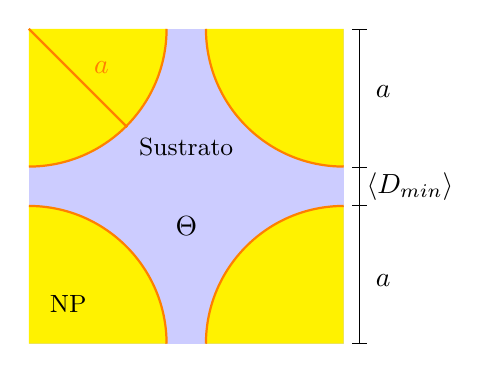
\begin{tikzpicture}[scale=1]
\def	\ll{2}
\def\a{1.75}
%------------------------------------------------ NPs and Substrate
\fill[blue!20] (-\ll,-\ll) rectangle (\ll,\ll);		

\fill[-,yellow,shift ={(-\ll,-\ll)}, opacity = 1](90:\a)arc(90:0:\a)--(0,0)--(90:\a);
\draw[-, orange, thick, shift ={(-\ll,-\ll)}](90:\a)arc(90:0:\a);

\fill[-,yellow,shift ={(-\ll,\ll)}, opacity = 1](-90:\a)arc(-90:0:\a)--(0,0)--(-90:\a);
\draw[-, orange, thick, shift ={(-\ll,\ll)}](-90:\a)arc(-90:0:\a);

\fill[-,yellow,shift ={(\ll,\ll)}, opacity = 1](-90:\a)arc(-90:-180:\a)--(0,0)--(-90:\a);
\draw[-, orange, thick, shift ={(\ll,\ll)}](-90:\a)arc(-90:-180:\a);

\fill[-,yellow,shift ={(\ll,-\ll)}, opacity = 1](90:\a)arc(90:180:\a)--(0,0)--(90:\a);
\draw[-, orange, thick, shift ={(\ll,-\ll)}](90:\a)arc(90:180:\a);

\draw[-, thick, orange] (-\ll,\ll)--(-\ll*.65,\ll*.65) node [anchor = south west]{$a$}--(-.75,.75);
%-------------------------------------------------- media names
\node at (0,.5) {\small Sustrato}; 
\node at (-1.5,-1.5) {\small NP};
\node at (0,-.5) {$\Theta$};

%--------------------------------------------------- dimensions
\draw[-|] (\ll+.2,\ll-\a)--(\ll+.2,\ll);
\node at (\ll+.5, \ll*.6){$a$};

\draw[-|] (\ll+.2,-\ll+\a)--(\ll+.2,-\ll);
\node at (\ll+.5,-\ll*.6){$a$};

\draw[|-|] (\ll+.2,\ll-\a)--(\ll+.2,-\ll+\a);
\node at (\ll+.5, 0){$\;\;\;\;\;\;\;\langle\mathscr{D}_{min}\rangle $};

\end{tikzpicture}
		\caption{ Vista superior de una monocapa de NPs de radio $a$ con fracción de cubierta $\Theta$ sobre un sustrato. La separación promedio entre las NPs es $\langle\mathscr{D}_{min}\rangle $, por lo que el área total del cuadrado es $(2a+\langle d \rangle)^2$, el de una NP es $\pi a^2$ y por tanto $\Theta= \pi a^2 / (2a+\langle\mathscr{D}_{min}\rangle )^2$.}\label{fig:MeanD}
	\end{figure}	
	
Al analizar  las Ecs. \eqref{eqs:rtcohSSA} y \eqref{eq:alpha} para ángulos rasantes $\theta\to \pi/2$, se observa que $\alpha\to \infty$, además de que para partículas pequeñas $x\ll 1$ el producto $r_{coh}^{SSA}r_{coh}^{SSA*}$ puede tomar valores mayores a la unidad. Por tanto, los coeficientes de amplitud calculados a partir de la SSA son válidos únicamente para ángulos de incidencia no rasantes  \cite{reyes2018analytical}.

Para calcular los coeficientes de amplitud de reflexión y transmisión para una monocapa de NPs que no estén limitados a ángulos de incidencia bajos, se deben considerar contribuciones de esparcimiento múltiple (Multiple Scattering, MS)\index{Esparcimiento!Múltiple (MS)!campo eléctrico esparcido promedio} en el cálculo del campo eléctrico $\vb{E}^{exc}$  que excita a las partículas dentro de la placa, el cual se puede descomponer como 
	\begin{align}
	\vb{E}^{exc} = \vb{E}^{exc}_{t} e^{i\vb{k}^t_{coh}\cdot\vb{r}}+
					\vb{E}^{exc}_{r} e^{i\vb{k}^r_{coh}\cdot\vb{r}},
	\end{align}
donde  $\vb{E}^{exc}_t$ es la componente del campo eléctrico que excita a las NPs que se transmite según la SSA y $\vb{E}^{exc}_{r}$ la que se refleja; dado que la reflexión y transmisión de $\vb{E}^{exc}$ están dadas por las Ecs. \eqref{eq:EsSSA}, su polarización es la de la onda plana $\vu{e}_i$ y su dirección de propagación está dada por $\vb{k}^t_{coh}$ y $\vb{k}^r_{coh}$, respectivamente. Entonces, el campo eléctrico esparcido promedio considerando el MS $\vb{E}^s_{MS}$, toma en cuenta  las reflexiones y transmisiones de $\vb{E}^{exc}$ según las Ecs. \eqref{eq:EsSSA} en el límite $d\to 0$ \cite{gutierrez2012overview}, como se observa en la Fig. \ref{fig:MScatt-slab-MS}, y la contribución del campo eléctrico incidente $\vb{E}^i$, por lo que  \cite{reyes2018analytical}
%
	\begin{subequations}\begin{align}
		\langle \vb{E}^s_{r,coh}\rangle & =	\langle \vb{E}^s_{r,\textit{MS}}\rangle
					= \qty[-\alpha S_j(\vartheta)E^{exc}_t -\alpha S(0)E^{exc}_r
					]\vu{e}_i e^{i\vb{k}^r_{coh}\cdot\vb{r}},\\
		\langle \vb{E}^s_{t,coh}\rangle & =\vb{E}^i+\langle\vb{E}^s_{t,\textit{MS}}\rangle
					= \qty[E_0 -\alpha S(0)E^{exc}_t 
					-\alpha	 S_j(\vartheta)E^{exc}_r
					]\vu{e}_i e^{i\vb{k}^t_{coh}\cdot\vb{r}}.
	\end{align} \label{eqs:EsMS}\end{subequations} \vspace*{-2em}

	\begin{figure}[h!]\centering
		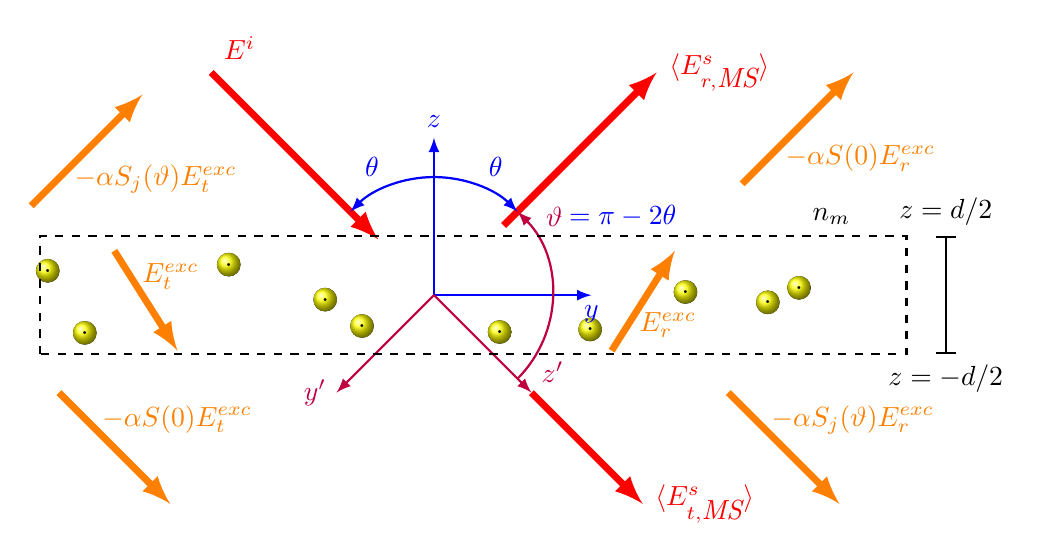
\begin{tikzpicture}[scale=1]
\def\a{.15}
\def\d{.75}

%----------------------NPs--------------
\foreach \y in {-4.5,-4.5,-2.5,-1.5,-.5,.5,1.5,3.5,4,4.5}{
\fill[ball color=yellow, opacity=1] (\y+rand*.5,rand*\d) circle(\a) node[ ]{.};
}

%----------------------averaged fields ---------------------
\draw[latex -, thick, red, line width=2.5](135:1)--(135:4) node[anchor=south west]{$\vb{E}^i$};
\draw[- latex, thick, red, line width=2.5](45:\d+.5)--(45:4)node[anchor=west]{$\langle\vb{E}_{r,\textit{MS}}^s\rangle$};
\draw[ - latex, thick, red, line width=2.5](-45:1.75)--(-45:3.75) node[anchor=west]{$\langle\vb{E}_{t,\textit{MS}}^s\rangle$};

%---------------------- Exciting fields ---------------------
\draw[- latex , thick,  orange, line width=2.5,shift ={(-3,0)}](152:1.2)node[anchor= north west]{$\;\;\vb{E}^{exc}_t$}--(250:\d);
\draw[latex - , thick, orange, line width=2.5,shift ={(2,0)}](28:1.2)--(-70:\d) node[anchor= south west]{$\;\;\vb{E}^{exc}_r$};

%-------------- reflected and transmitted exciting fields DOWN ---------------------
\draw[latex - , thick, orange, line width=2.5,shift={(2.5, 0)}](-45:3.75)--(-45:1.75) node[anchor=north west]{$\;\;\;\;-\alpha S_j(\vartheta)\vb{E}^{exc}_r$};
\draw[latex - , thick, orange, line width=2.5,shift={(-6, 0)}](-45:3.75)--(-45:1.75) node[anchor=north west]{$\;\;\;\;-\alpha S(0)\vb{E}^{exc}_t$};

%-------------reflected and transmitted exciting fields UP ---------------------
\draw[latex -, thick, orange, line width=2.5,shift={(2.5, 0)}](45:4)--(45:2)node[anchor=south west]{$\;\;\;\;-\alpha S(0) \vb{E}^{exc}_r$};
\draw[latex -, thick, orange, line width=2.5,shift={(-6, .25)}](45:3.25)--(45:\d+.5)node[anchor=south west]{$\;\;\;\;-\alpha S_j(\vartheta) \vb{E}^{exc}_t$};

%----------------------main system---------------------
\draw[- latex, thick, blue] (0,0)--(90:2) node[anchor = south]{$z$};
\draw[- latex, thick, blue] (0,0)--(0:2) node[anchor = north]{$y$};
\path (0,0)++(135/2:1.5)node[anchor=south west, blue]{$\theta$}; 
\draw[- latex, thick, blue](90:1.5)arc(90:45:1.5);
\path (0,0)++(90+45/2:1.5)node[anchor=south east, blue]{$\theta$}; 
\draw[- latex, thick, blue](90:1.5)arc(90:135:1.5);

%----------------------Mie system---------------------
\draw[- latex, thick, purple] (0,0)--(-45:1.75) node[anchor = south west]{$z'$};
\draw[- latex, thick, purple] (0,0)--(-135:1.75) node[anchor = east]{$y'$};
\path (0,0)++(30:1.5)node[anchor=south west, purple]{$\vartheta$}; 
\path (0,0)++(30:1.5)node[anchor=south west, blue]{$\;\;\; =  \pi - 2\theta$}; 
\draw[- latex, thick, purple](-45:1.5)arc(-45:45:1.5);

%----------------------thickness and slab ---------------------
\draw[thick, dashed] (-5,-\d) rectangle (6,\d);
%\draw[thick, dashed] (-5, 0) --  (6,0);
\draw[ |-|, thick,] (6.5,-\d) node[anchor = north]{$z=-d/2$} -- (6.5,\d) node[anchor = south]{$z=d/2$};
\node at (5,1) {$\; n_m$};
\end{tikzpicture}
		\caption{ Película de grosor $d$ y volumen $V$ con $N$ partículas esféricas idénticas excitada por una onda plana monocromática incidente en la dirección $\vb{k}^i$. El campo eléctrico que excita a las NPs dentro de la película $\vb{E}^{exc}$ se divide en una componente reflejada $ \vb{E}^{exc}_r$ y una transmitida $ \vb{E}^{exc}_t$, considerando así el esparcimiento múltiple por las NPs. Los campos eléctricos esparcidos promedio reflejado $\langle \vb{E}^s_{r,coh}\rangle$ y transmitido $\langle \vb{E}^s_{r,coh}\rangle$ corresponden a la suma  de las Ecs. \eqref{eqs:rtcohSSA} aplicadas a $\vb{E}^{exc}_t$ y a $\vb{E}^{exc}_r$ como se representa en la figura y en las Ecs. \eqref{eqs:EsMS}. Las flechas rojas corresponden a la onda plana incidente y los campos esparcidos promedios mientras que las flechas naranjas corresponden al campo que excita a las NPs. }\label{fig:MScatt-slab-MS}
	\end{figure}	
	
Para determinar la expresión del campo eléctrico que excita a las NPs en la placa $\vb{E}^{exc}$ considerando el MS\footnote{El procedimiento descrito emplea un enfoque heurístico que se publicó en \cite{reyes2018analytical} sin emabargo, un enfoque más riguroso se encuentra en \cite{barrera2003coherent}.}, se divide la placa donde se encuentras las NPs en dos (de grosor $d/2$ cada una) y se calcula el promedio de  $\vb{E}^{exc}$ en la interfaz entre las dos placas ($z=0$) de forma autoconsistente, por lo que las NPs en la placa no sólo son iluminadas por el campo eléctrico incidente $\vb{E}^i$, sino también por $\vb{E}^{exc}$ \cite{reyes2018analytical}. La componente de $\vb{E}^{exc}$ que se transmite, $\vb{E}^{exc}_{t}$, se calcula como la suma del campo eléctrico incidente más el promedio de la transmisión del campo $E^{exc}_t$ y a la reflexión del campo $E^{exc}_r$ ---que corresponden a la suma de los campos esparcidos por las NPs en la placa superior ($0<z<d/2$)--- , es decir,
%
	\begin{subequations}\begin{align}
		\vb{E}^{exc}_t  e^{i\vb{k}^i\cdot\vb{r}}  =
				\qty[E_0  - \frac12 \qty(
					\alpha S(0)E^{exc}_t + \alpha S_j(\vartheta)E^{exc}_r
				)] e^{i\vb{k}^t_{coh}\cdot\vb{r}}  \vu{e}_i,
	\end{align}
%
donde el factor $1/2$ indica que es la respuesta EM promedio dentro de la placa. Asimismo, el campo $\vb{E}^{exc}_{r}$ se calcula como la reflexión  del campo $E^{exc}_t$ y la transmisión del campo $E^{exc}_r$ ---campos esparcidos por las NPs en la placa inferior ($-d/2<z<0$)---, por lo que su expresión es	
%
	\begin{align}
	\vb{E}^{exc}_r  e^{i\vb{k}^r\cdot\vb{r}}  =
				\qty[- \frac12 \qty(
					\alpha S_j(\vartheta)E^{exc}_t + \alpha S(0)E^{exc}_r
				)] e^{i\vb{k}^r_{coh}\cdot\vb{r}}  \vu{e}_i.
	\end{align} \label{eq:Eexc}\end{subequations}
%
En la Fig. \ref{fig:Eexc} se muestra una representación gráfica de las Ecs. \eqref{eq:Eexc}, que son válidas únicamente en $-d/2<z<d/2$.

\begin{figure}[h!]\centering
	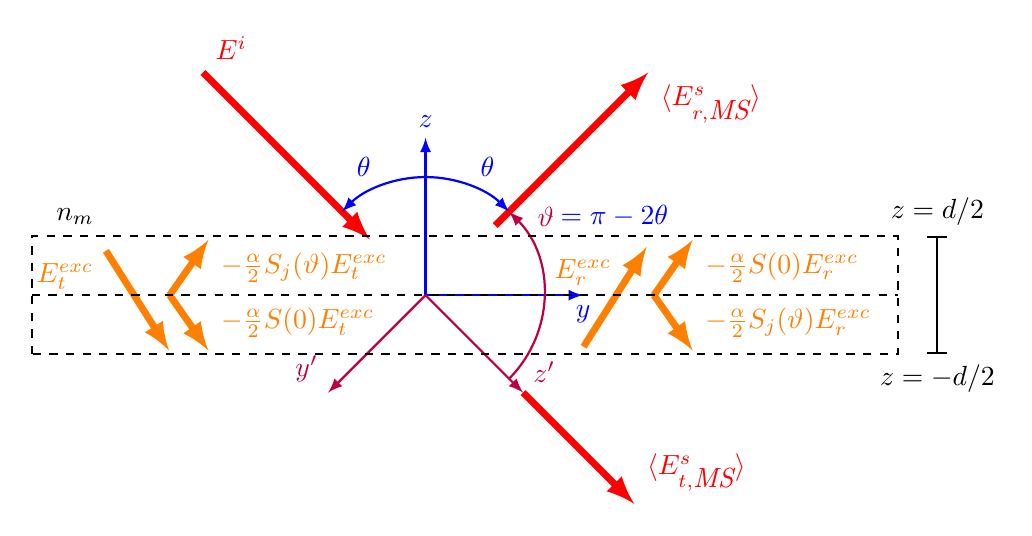
\begin{tikzpicture}[scale=1]
\def\a{.15}
\def\d{.75}

%\foreach \y in {-4.5,-3.5,-2.5,-.5,.5,2.5,3.5,4.5}{
%\fill[ball color=yellow, opacity=1] (\y+rand*.5,rand*\d) circle(\a) node[ ]{.};
%}


\draw[latex -, thick, red, line width=2.5](135:1)--(135:4) node[anchor=south west]{$\vb{E}^i$};
\draw[- latex, thick, red, line width=2.5](45:\d+.5)--(45:4)node[anchor=north west]{$\langle\vb{E}_{r,\textit{MS}}^s\rangle$};
\draw[ - latex, thick, red, line width=2.5](-45:1.75)--(-45:3.75) node[anchor=south west]{$\langle\vb{E}_{t,\textit{MS}}^s\rangle$};

%---------------------- Exciting transmitted field ---------------------
\draw[latex - , thick,  orange, line width=2.5,shift={(-3., 0)}](250:\d)--(152:1.2) node[anchor= north east]{$\vb{E}^{exc}_t$};

\draw[- latex , thick,  orange, line width=2.5, shift={(-2.5, 0)}](180:\d)--(250:\d) node[anchor= south west]{$-\frac{\alpha}{2} S(0)\vb{E}^{exc}_t$};
\draw[- latex , thick,  orange, line width=2.5, shift={(-2.5, 0)}](180:\d)--(110:\d) node[anchor= north west]{$-\frac{\alpha}{2} S_j(\vartheta)\vb{E}^{exc}_t$};

%---------------------- Exciting reflected field ---------------------
\draw[- latex , thick, orange, line width=2.5,shift={(1.75, .05)}](-70:\d)--(28:1.2) node[anchor=north east]{$\vb{E}^{exc}_r\;\;\;$};

\draw[- latex , thick,  orange, line width=2.5, shift={(3.65, 0)}](180:\d)--(250:\d) node[anchor= south west]{$-\frac{\alpha}{2} S_j(\vartheta)\vb{E}^{exc}_r$};
\draw[- latex , thick,  orange, line width=2.5, shift={(3.65, 0)}](180:\d)--(110:\d) node[anchor= north west]{$-\frac{\alpha}{2}S(0)\vb{E}^{exc}_r$};

%----------------------Main system---------------------
\draw[- latex, thick, blue] (0,0)--(90:2) node[anchor = south]{$z$};
\draw[- latex, thick, blue] (0,0)--(0:2) node[anchor = north]{$y$};
\path (0,0)++(135/2:1.5)node[anchor=south west, blue]{$\theta$}; 
\draw[- latex, thick, blue](90:1.5)arc(90:45:1.5);
\path (0,0)++(90+45/2:1.5)node[anchor=south east, blue]{$\theta$}; 
\draw[- latex, thick, blue](90:1.5)arc(90:135:1.5);

%----------------------Mie system---------------------
\draw[- latex, thick, purple] (0,0)--(-45:1.75) node[anchor =south west]{$z'$};
\draw[- latex, thick, purple] (0,0)--(-135:1.75) node[anchor =south east]{$y'$};
\path (0,0)++(30:1.5)node[anchor=south west, purple]{$\vartheta$}; 
\path (0,0)++(30:1.5)node[anchor=south west, blue]{$\;\;\; =  \pi - 2\theta$}; 
\draw[- latex, thick, purple](-45:1.5)arc(-45:45:1.5);

%----------------------thickness and slab ---------------------
\draw[thick, dashed] (-5,-\d) rectangle (6,\d);
\draw[thick, dashed] (-5, 0) --  (6,0);
\draw[ |-|, thick,] (6.5,-\d) node[anchor = north]{$z=-d/2$} -- (6.5,\d) node[anchor = south]{$z=d/2$};
\node at (-4.5,1) {$\; n_m$};

\end{tikzpicture}
	\caption{ Película de grosor $d$ y volumen $V$ con $N$ partículas esféricas idénticas (no mostradas en la figura) divida en dos regiones: $z<0$ y $z>0$. Una onda plana monocromática propagándose en la dirección $\vb{k}^i$ incide en las placas, generando un campo eléctrico que excita a las NPs dentro de la película y que considera el esparcimiento múltiple de las NPs al dividirlo en una componente reflejada $\vb{E}^{exc}_r$ y una transmitida $\vb{E}^{exc}_t$, dando como resultado a los campos esparcidos promedio reflejado $\langle\vb{E}_{r,\textit{MS}}^s\rangle$ y transmitido $\langle\vb{E}_{t,\textit{MS}}^s\rangle$. Sobre la interfaz entre las dos placas ($z=0$) tanto $\vb{E}^{exc}_r$ como $\vb{E}^{exc}_t$ se reflejan y transmiten según las Ecs. \eqref{eqs:rtcohSSA}, proceso descrito por las Ecs. \eqref{eq:Eexc}. Las flechas rojas corresponden a la onda plana incidente y los campos esparcidos promedios mientras que las flechas naranjas corresponden al campo que excita a las NPs. }\label{fig:Eexc}
	\end{figure}	
	
Al resolver las Ecs. \eqref{eq:Eexc} para $E^{exc}_t$ y $E^{exc}_r$ en términos del campo eléctrico incidente $\vb{E}_0$ se obtienen las siguientes expresiones
%
	\begin{align*}
	\vb{E}^{exc}_t  &= \frac{1+\frac12\alpha S(0)}
				{1+\alpha S(0) +\frac14\alpha^2\qty[S^2(0)-S_j^2(\vartheta)]}\vb{E}_0,\\
	\vb{E}^{exc}_r  &= \frac{-\frac12\alpha S_j(\vartheta)}
				{1+\alpha S(0) +\frac14\alpha^2\qty[S^2(0)-S_j^2(\vartheta)]}\vb{E}_0,
	\end{align*}
%
por lo que, al sustituirlas en las expresiones de los campos esparcidos promedio reflejados y transmitidos [Ecs. \eqref{eqs:EsMS}], se obtienen
%
	\begin{align*}
	\langle \vb{E}^s_{r,coh}\rangle &=
			\frac{-\alpha S_j(\vartheta)}{1+\alpha S(0)+\frac14 \alpha^2 \left[S^2(0)-S_j^2 (\vartheta) \right]} \vb{E}_0 e^{i\vb{k}^r_{coh}\cdot\vb{r}},\\
	\langle \vb{E}^s_{r,coh}\rangle &=
			\frac{1-\frac14\alpha^2\qty[S^2(0)-S_j^2(\vartheta)]}{1+\alpha S(0)+\frac14 \alpha^2 \left[S^2(0)-S_j^2 (\vartheta) \right]} \vb{E}_0 e^{i\vb{k}^t_{coh}\cdot\vb{r}},
	\end{align*}
%
de donde es posible calcular los coeficientes de amplitud de reflexión y transmisión para una monocapa de NPs esféricas bajo el formalismo del CSM. Entonces, considerando que el campo eléctrico que excita a las NPs toma en cuenta el esparcimiento múltiple y que la componente coherente del campo esparcido es mucho mayor que la contribución de la componente difusa, así como $\vartheta = \pi-2\theta$, se obtiene que\index{Esparcimiento!Coherente, Modelo de (CSM)!coeficientes de amplitud! para una monocapa en espacio libre} \vspace*{-.75em}
%
	\begin{subequations}\begin{tcolorbox}[title = Coeficientes de amplitud del CSM, breakable ]
	\begin{align}
	r_{coh}&=\frac{-\alpha S_j(\pi-2\theta)}
				{1+\alpha S(0)+\frac14 \alpha^2 \left[S^2(0)-S_j^2 (\pi-2\theta) \right]},
			\label{seq:rcoh}\\
	t_{coh}&=\frac{1-\frac14\alpha^2\qty[S^2(0)-S_j^2(\pi-2\theta)]}
				{1+\alpha S(0)+\frac14 \alpha^2 \left[S^2(0)-S_j^2 (\pi-2\theta) \right]},
		\label{seq:tcoh}
	\end{align}
	con $j=1$ para polarización $s$, $j=2$ para $p$ y $S(0)=S_1(0)=S_2(0)$.
	\end{tcolorbox}\label{eqs:rtcoh}\end{subequations}\vspace*{-.75em}\noindent

	 \subsection{Monocapa sobre un sustrato}

Las Ecs. \eqref{eqs:rtcoh} corresponden a los coeficientes de amplitud de reflexión y transmisión de una onda plana $\vb{E}^i$ que incide a un ángulo $\theta$ sobre una monocapa de NPs esféricas, idénticas, de radio $a$ e índice de refracción $n_p$, localizadas de forma aleatoria e inmersa en una matriz con índice de refracción $n_m$, sin ser soportada de alguna forma. Sin embargo, en la realidad las NPs no pueden estar suspendidas en un espacio libre, sino que están soportadas sobre un sustrato, de índice de refracción $n_s$; adicionalmente la incidencia del haz de luz puede ser tanto en configuración externa, como se muestra en la Fig. \ref{figs:CSM-Ext}, como en interna, es decir ATR, como se muestra en la Fig. \ref{figs:CSM-ATR}.

	\begin{figure}[h!]\centering
	\begin{subfigure}{.05\textwidth}\vspace{-4.5cm}\caption{}\label{figs:CSM-Ext}\end{subfigure}\hspace*{-2em}
	\begin{subfigure}{.48\textwidth}
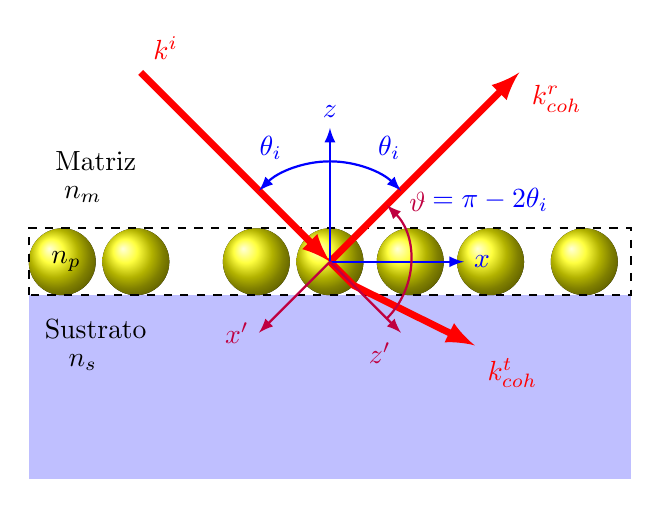
\begin{tikzpicture}[scale=.85]
\def\a{. 5}
\def\d{. 5}

\fill[blue, opacity=. 25] (-4. 5,-6.5*\d) rectangle (4. 5,-\d);

\foreach \x in {-4,-2. 9,-1. 1,0,1. 2,2. 4,3. 8}{
\fill[ball color=yellow, opacity=1] (\x,0) circle(\a);}


\draw[thick, dashed] (-4. 5,-\d) rectangle (4. 5,\d);

\draw[latex -, thick, red, line width=2. 5](135:0)--(135:4) node[anchor=south west]{$\vb{k}^i$};
\draw[- latex, thick, red, line width=2. 5](135:0)--(135:-.5)--(150:-2.5) node[anchor=north west]{$\vb{k}^t_{coh}$};
\draw[- latex, thick, red, line width=2. 5](45:0)--(45:4)node[anchor=north west]{$\vb{k}^r_{coh}$};

\draw[- latex, thick, blue] (0,0)--(90:2) node[anchor = south]{$z$};
\draw[- latex, thick, blue] (0,0)--(0:2) node[anchor = west]{$x$};
\path (0,0)++(135/2:1. 5)node[anchor=south west, blue]{$\theta_i$}; 
\draw[- latex, thick, blue](90:1. 5)arc(90:45:1. 5);
\path (0,0)++(90+45/2:1. 5)node[anchor=south east, blue]{$\theta_i$}; 
\draw[- latex, thick, blue](90:1. 5)arc(90:135:1. 5);

\draw[- latex, thick, purple] (0,0)--(-45:1. 5) node[anchor = north east]{$z'$};
\draw[- latex, thick, purple] (0,0)--(-135:1. 5) node[anchor = east]{$x'$};
\path (0,0)++(30:1. 2)node[anchor=south west, purple]{$\vartheta$}; 
\path (0,0)++(30:1. 2)node[anchor=south west, blue]{$\;\;\; =  \pi - 2\theta_i$}; 
\draw[- latex, thick, purple](-45:1. 2)arc(-45:45:1. 2);



\node at (-3.5,1.5) {Matriz};
\node at (-3.75,1) {$\; n_m$};
\node at (-4,0) {$\; n_p$};
\node at (-3.75,-1.5) {$\; n_s$};
\node at (-3.5,-1) {Sustrato};	
\end{tikzpicture}
	\end{subfigure}
	\begin{subfigure}{.05\textwidth}\vspace{-4.5cm}\caption{}\label{figs:CSM-ATR}	\end{subfigure}\hspace*{-2em}
	\begin{subfigure}{.48\textwidth} 
		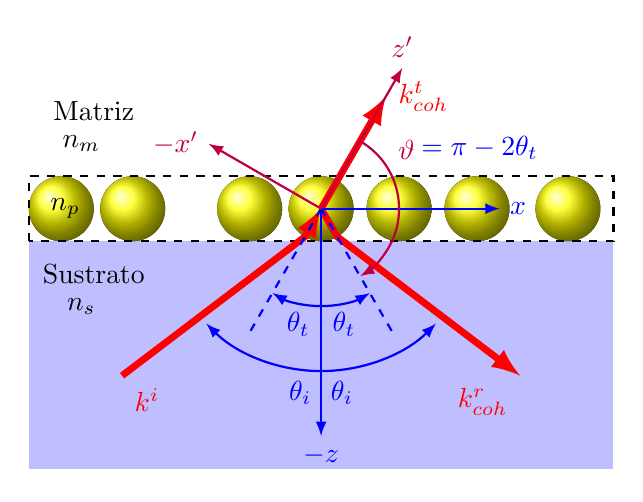
\begin{tikzpicture}[scale=.825]
\def\a{. 5}
\def\d{. 5}

\fill[blue, opacity=. 25] (-4. 5,-8*\d) rectangle (4. 5,-\d);

\foreach \x in {-4,-2. 9,-1. 1,0,1. 2,2. 4,3. 8}{
\fill[ball color=yellow, opacity=1] (\x,0) circle(\a);}


\draw[thick, dashed] (-4. 5,-\d) rectangle (4. 5,\d);

\draw[latex -, thick, red, line width=2. 5](0,0)--(-120:. 5)--(-140:4) node[anchor=north west]{$\vb{k}^i$};
\draw[- latex, thick, red, line width=2. 5](0,0)--(-120:-2)node[anchor=west]{$\vb{k}^t_{coh}$};
\draw[- latex, thick, red, line width=2. 5](0,0)--(-60:. 5)--(-40:4)node[anchor=north east]{$\vb{k}^r_{coh}$};

\draw[- latex, thick, blue] (0,0)--(-90:3. 5) node[anchor = north]{$-z$};
\draw[- latex, thick, blue] (0,0)--(0:2. 75) node[anchor = west]{$x$};

\path (0,0)++(-90:2. 5)node[anchor=north east, blue]{$\theta_i$}; 
\draw[- latex, thick, blue](-90:2. 5)arc(-90:-45:2. 5);
\path (0,0)++(-90:2. 5)node[anchor=north west, blue]{$\theta_i$}; 
\draw[- latex, thick, blue](-90:2. 5)arc(-90:-135:2. 5);

\draw[thick, blue, dashed](0,0) -- (-120:2. 25);
\draw[thick, blue, dashed](0,0) -- (-60:2. 25);
\path (0,0)++(-90-50/2:1. 6)node[anchor=north west, blue]{$\theta_t$}; 
\draw[- latex, thick, blue](-90:1. 5)arc(-90:-60:1. 5);
\path (0,0)++(-90+50/2:1. 6)node[anchor=north east, blue]{$\theta_t$}; 
\draw[- latex, thick, blue](-90:1. 5)arc(-90:-120:1. 5);

\draw[- latex, thick, purple] (0,0)--(60:2.5) node[anchor = south]{$z'$};
\draw[- latex, thick, purple] (0,0)--(150:2) node[anchor =  east]{$-x'$};
\path (0,0)++(30:1. 2)node[anchor=south west, purple]{$\vartheta$}; 
\path (0,0)++(30:1. 2)node[anchor=south west, blue]{$\;\;\; =  \pi - 2\theta_t$}; 
\draw[- latex, thick, purple](60:1. 2)arc(60:-60:1. 2);


\node at (-3.5,1.5) {Matriz};
\node at (-3.75,1) {$\; n_m$};
\node at (-4,0) {$\; n_p$};
\node at (-3.75,-1.5) {$\; n_s$};
\node at (-3.5,-1) {Sustrato};	
\end{tikzpicture}
	\vspace*{-.35em}\end{subfigure}
	\caption{Esquema de la reflexión coherente de una monocapa de NPs esféricas, con índice de refracción $n_p$,  suspendida en una matriz con índice de refracción $n_m$ y soportada por un sustrato con índice de refracción $n_s$, iluminada en un esquema de \textbf{a)} incidencia externa  y \textbf{b)} en configuración ATR. El sistema coordenado azul, con el eje $z$ paralelo a la dirección normal a la monocapa, define los ángulos de incidencia $\theta_i$, de reflexión y de transmisión $\theta_t$ mediante la ley de la reflexión y la ley de Snell. El sistema coordenado morado, con el eje $z$ paralelo a $\vb{k}^i$ en \textbf{a)} y paralelo a $\vb{k}^t_{coh}$ en \textbf{b)}, se emplea para determinar el ángulo $\vartheta$ (donde se evalúan los elmentos de la matriz de esparcimiento de Mie) en términos de $\theta_i$ o $\theta_t$.}	\label{fig:CSM-Diagrams}	
	\end{figure}	

En la Fig. \ref{fig:CSM-Diagrams}	 se observa que el ángulo $\theta$ a evaluar $r_{coh}$ y $t_{coh}$ en las Ecs. \eqref{eqs:rtcoh} depende del medio por el que incide el campo eléctrico de la onda plana, con dirección $\vb{k}^i$. En incidencia externa, Fig. \ref{figs:CSM-Ext}, la onda plana incide sobre las NPs a un ángulo $\theta_i$ dado que no interactúa con la interfaz matriz-sustrato y no modifica su trayectoria. Por otro lado, en una configuración ATR, Fig. \ref{figs:CSM-ATR}, la onda plana cruza la interfaz sustrato-matriz, por lo que se refracta a un ángulo $\theta_t$ dado por la ley de Snell, e incide a la monocapa en $\theta=\theta_t$. Además de considerar el ángulo con el que la onda plana ilumina a las NPs, se debe calcular la contribución del sustrato en la reflectancia $R$ y transmitancia $T$, que también depende del medio por donde incide la onda plana.

\begin{figure}[b!]\centering
	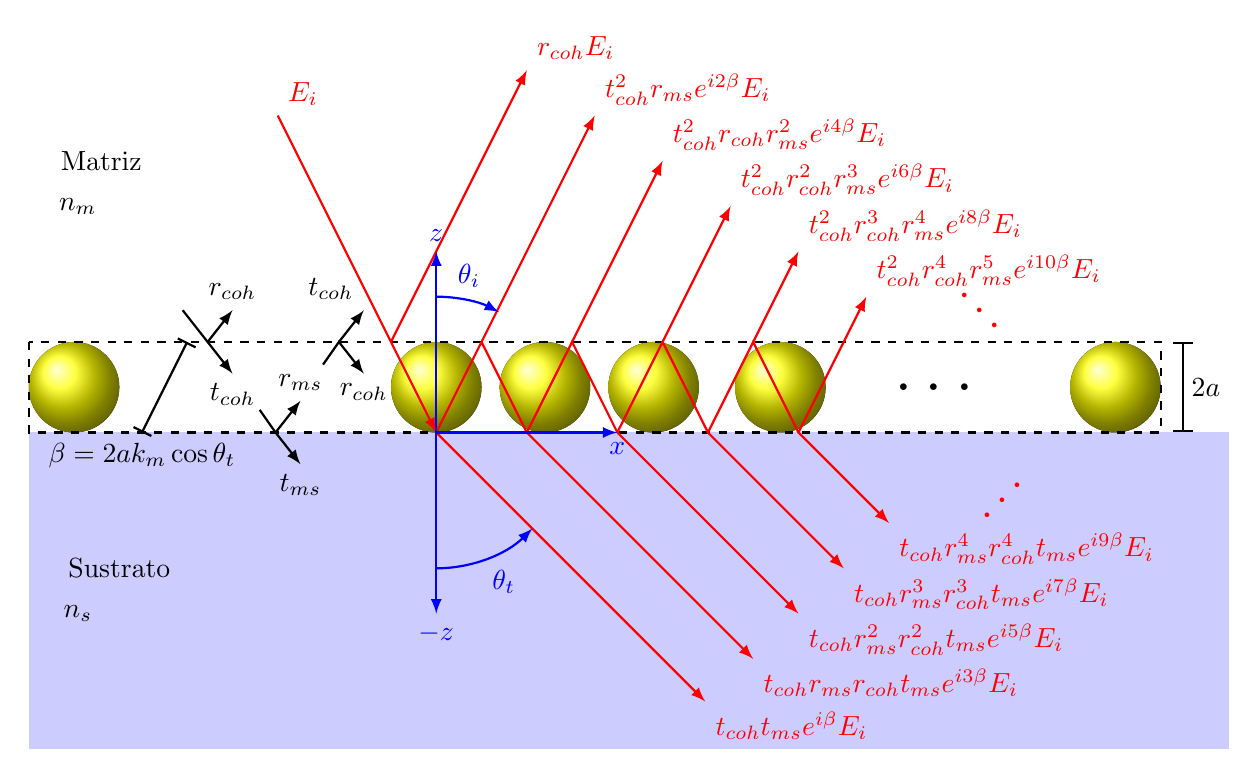
\begin{tikzpicture}[scale=1.15]
\def\a{.5}
\def\d{.5}
\def\t{.3}

\fill[blue, opacity = .2] (-4.5,-3.5) rectangle(8.75,0);

\foreach \x in {-4,0,1.2,2.4,3.8,7.5}{ %-2.9,-1.1
\fill[ball color=yellow, opacity=1] (\x,\d) circle(\a);}

\draw[thick, dashed] (-4.5,2*\d) rectangle (8,0);
\node at (5.5,\d) {\Huge $\ldots$};

%%%%%%%%%%%%%-------------transmisiones

\draw[- latex, thick, red](-135:0)--(-45:4.2) node[anchor=north west]{$t_{coh}t_{ms}e^{i\beta}E_i$};
\draw[- latex, thick, red](0,0)--(1*\d,2*\d)--(2*\d,0)--(3+\d,-3+\d) node[anchor=north west]{$t_{coh}r_{ms}r_{coh}t_{ms}e^{i3\beta}E_i$};
\draw[- latex, thick, red](2*\d,0)--(3*\d,2*\d)--(4*\d,0)--(3+2*\d,-3+2*\d) node[anchor=north west]{$t_{coh}r_{ms}^2r_{coh}^2t_{ms}e^{i5\beta}E_i$};
\draw[- latex, thick, red](4*\d,0)--(5*\d,2*\d)--(6*\d,0)--(3+3*\d,-3+3*\d) node[anchor=north west]{$t_{coh}r_{ms}^3r_{coh}^3t_{ms}e^{i7\beta}E_i$};
\draw[- latex, thick, red](6*\d,0)--(7*\d,2*\d)--(8*\d,0)--(3+4*\d,-3+4*\d) node[anchor=north west]{$t_{coh}r_{ms}^4r_{coh}^4t_{ms}e^{i9\beta}E_i$};
\draw[-, thick, red](8*\d,0)--(9*\d,2*\d);
\node[rotate={45}] at (6.25,-.75) {\color{red}\LARGE $\ldots$};


%%%%%%%%%%%%%-------------reflexiones
\draw[latex -, thick, red](0,0)--(-1.75,3.5) node[anchor=south west]{$E_i$};
\draw[- latex, thick, red](-1*\d,2*\d)--(2-2*\d,4+0*\d) node[anchor=south west]{$r_{coh}E_i$};
\draw[- latex, thick, red](1*\d,2*\d)--(1.75,3.5) node[anchor=south west]{$t_{coh}^2r_{ms}e^{i2\beta}E_i$};
\draw[- latex, thick, red](3*\d,2*\d)--(2+1*\d,4-2*\d) node[anchor=south west]{$ t_{coh}^2r_{coh}r_{ms}^2e^{i4\beta}E_i$};
\draw[- latex, thick, red](5*\d,2*\d)--(2+2.5*\d,4-3*\d) node[anchor=south west]{$ t_{coh}^2r_{coh}^2r_{ms}^3e^{i6\beta}E_i$};
\draw[- latex, thick, red](7*\d,2*\d)--(2+4*\d,4-4*\d) node[anchor=south west]{$ t_{coh}^2r_{coh}^3r_{ms}^4e^{i8\beta}E_i$};
\draw[- latex, thick, red](9*\d,2*\d)--(2+5.5*\d,4-5*\d) node[anchor=south west]{$t_{coh}^2r_{coh}^4r_{ms}^5e^{i10\beta}E_i$};
\node[rotate={-45}] at (6,1.35) {\color{red}\LARGE $\ldots$};



\node at (-4,2.5) {$\; n_m$};
\node at (-3.7,3) {Matriz};
\node at (-4,-2) {$\; n_s$};
\node at (-3.5,-1.5) {Sustrato};

%.55,0
%2,0
%1.2,2*\ḑ
%%\draw[latex - , thick](-2.8,-.5)--(-3.5,.5) node[anchor=north]{$r_{sm},\,t_{sm}$};
\draw[latex - , thick, shift ={(2,2*\d)}](-2.8,-.35)node[anchor=north]{$r_{coh}$}--(-3.075,0)--(-3.25,-.25);
\draw[latex -,thick, shift ={(2,2*\d)}](-2.8,.35)node[anchor=south east]{$t_{coh}$}--(-3.075,0);
\draw[latex - , thick, shift ={(.55,2*\d)}](-2.8,-.35)node[anchor=north]{$t_{coh}$}--(-3.075,0)--(-3.35,.35);
\draw[latex -,thick, shift ={(.55,2*\d)}](-2.8,.35)node[anchor=south]{$r_{coh}$}--(-3.075,0);
\draw[latex - , thick, shift ={(1.3,0)}](-2.8,-.35)node[anchor=north]{$t_{ms}$}--(-3.075,0)--(-3.25,+.25);
\draw[latex -,thick, shift ={(1.3,0)}](-2.8,.35)node[anchor=south]{$r_{ms}$}--(-3.075,0);

\draw[|-|,thick, shift ={(-3.25,0)}](0,0)node[anchor=north]{$\beta = 2ak_m\cos\theta_t$}--(1*\d,2*\d) ;

\draw[|-|,thick, shift ={(8.25,0)}](0,0)--(0,2*\d) ;
\node at (8.5,\d){$2a$};

\draw[- latex, thick, blue] (0,0)--(90:2) node[anchor = south]{$z$};
\draw[- latex, thick, blue] (0,0)--(90:-2) node[anchor = north]{$-z$};
\draw[- latex, thick, blue] (0,0)--(0:2) node[anchor = north]{$x$};
\path (0,0)++(85:1.5)node[anchor=south west, blue]{$\theta_i$}; 
\draw[- latex, thick, blue](90:1.5)arc(90:62.5:1.5);
\path (0,0)++(-70:1.5)node[anchor=north west, blue]{$\theta_t$}; 
\draw[- latex, thick, blue](-90:1.5)arc(-90:-45:1.5);


\end{tikzpicture}
	\caption{ Esquema de las múltiples reflexiones en incidencia externa del sistema matriz-monocapa-sustrato producidos por una onda plana $\vb{E}^i$ que incide sobre una monocapa de NPs esféricas de radio $a$, inmersa en una matriz con índice de refracción  $n_m$ y soportada por un sustrato con índice de refracción $n_s$, a un ángulo $\theta_i$ respecto a la dirección normal de la monocapa. Las reflexiones y transmisiones en la interfaz sustrato-matriz ($z=0$) se describen mediante los coeficientes de amplitud de Fresnel [Ecs. \eqref{eq:rs}--\eqref{eq:tp}], mientras que en la interfaz monocapa-matriz ($z=2a$) las reflexiones y transmisiones son descritas por el CSM [Ecs. \eqref{eqs:rtcoh}]. Los coeficientes de amplitud de reflexión y transmisión se evalúan en $\theta_i$. En los coeficientes de amplitud  $r_{\alpha\beta}$ y $t_{\alpha\beta}$ el medio de incidencia de la onda plana monocromática corresponde a $\alpha$ y el de transmisión a $\beta$.}\label{fig:CSM-externa}
	\end{figure}

Para calcular los coeficientes de amplitud de reflexión y transmisión del sistema matriz-monocapa-sustrato, es decir, en incidencia externa, se consideran las múltiples reflexiones del sistema, mostradas en la Fig. \ref{fig:CSM-externa}. Cuando la onda plana con amplitud $E_i$ incide en la monocapa, en $z=2a$, se presenta una primera reflexión dada por el CSM, es decir que la amplitud del campo eléctrico en la primera reflexión es $r_{coh}E_i$. La segunda reflexión se presenta tras dos transmisiones en la monocapa y una reflexión en la interfaz matriz-sustrato, con una diferencia de fase $2\beta=2(2ak_m\cos\theta)$ respecto a la primera reflexión, es decir, que la amplitud de la segunda reflexión es $t_{coh}^2r_{ms}e^{i2\beta}E_i$. En la tercera reflexión hay dos transmisiones en la monocapa, dos reflexiones en la interfaz matriz-sustrato, y una reflexión en la monocapa; al considerar la diferencia de camino óptico con la primera relfexión, la amplitud de la tercera reflexión es $t_{coh}^2r_{coh}r_{ms}^2e^{i4\beta}E_i$. Al considerar el resto de las reflexiones, se obtiene que el coeficiente de amplitud de reflexión $r$ del sistema es \index{Fresnel!coeficientes de amplitud de ($r,t$)}
%
	\begin{align}
	r = r_{coh} +
		 t_{coh}^2r_{ms}e^{i2\beta}+
		 t_{coh}^2r_{coh}r_{ms}^2e^{i4\beta}+
		 t_{coh}^2r_{coh}^2r_{ms}^3e^{i6\beta}+
		 t_{coh}^2r_{coh}^3r_{ms}^4e^{i8\beta}+\ldots
%		 t_{coh}^2r_{coh}^4r_{ms}^5e^{i10\beta}+\ldots\,.
	\label{eq:r_ext_span}
	\end{align}
%
Para el cálculo del coeficiente de amplitud de transmisión $t $ del sistema se sigue un procedimiento análogo al de $r$: la primera transmisión ocurre después de una transmisión en la monocapa, una transmisión en la interfaz matriz-sustrato y una diferencia de fase de $\beta$, por lo que la amplitud de la primera transmisión es $t_{coh}t_{ms}e^{i\beta}$. Para la $m$-ésima transmisión se presentan $m-1$ reflexiones con la monocapa y $m-1$ con el sustrato, además de una fase de $(2m-1)\beta$, es decir,
%
	\begin{align}
	t = t_{coh}t_{ms}e^{i\beta} +
		t_{coh}r_{ms}r_{coh}t_{ms}e^{i3\beta}+
		t_{coh}r_{ms}^2r_{coh}^2t_{ms}e^{i5\beta}+	
		t_{coh}r_{ms}^3r_{coh}^3t_{ms}e^{i7\beta}+ \ldots					
%		t_{coh}r_{ms}^4r_{coh}^4t_{ms}e^{i9\beta}+ \ldots				
%		t_{coh}r_{ms}^5r_{coh}^5t_{ms}e^{i11\beta}+\ldots\,.
	\label{eq:t_ext_span}
	\end{align}\noindent
%	
Al factorizar $r_{ms}t_{coh}^2e^{2i\beta}$ en la Ec. \eqref{eq:r_ext_span}, a excepción del primer término $r_{coh}$, y factorizar $t_{coh}t_{ms}e^{i\beta}$ en la Ec. \eqref{eq:t_ext_span}, se obtienen las siguientes expresiones
%
	\begin{align*}
	r &= r_{coh} + r_{ms}t_{coh}^2e^{2i\beta}\left[1+r_{coh}r_{ms}e^{2i\beta}+\qty(r_{coh}r_{ms}e^{2i\beta})^2+\qty(r_{coh}r_{ms}e^{2i\beta})^3+\ldots,\right]\\
	t &= t_{coh}t_{ms}e^{i\beta} \left[1+r_{coh}r_{ms}e^{2i\beta}+\qty(r_{coh}r_{ms}e^{2i\beta})^2+\qty(r_{coh}r_{ms}e^{2i\beta})^3+\ldots\right] ,
	\end{align*}
%
y dado que $\norm{r_{coh}r_{ms}e^{2i\beta}}<1$, es posible reescribir los coeficientes de amplitud del sistema como\index{Esparcimiento!Coherente, Modelo de (CSM)!coeficientes de amplitud!incidencia externa)} \vspace*{-.75em}\begin{subequations}
%
	\begin{tcolorbox}[title = Coeficientes de amplitud dados por el CSM en incidencia externa, breakable ]
	\eqhalf{r = r_{coh}(\theta_i)+ \frac{r_{ms}(\theta_i)t_{coh}(\theta_i)e^{i2\beta}}
										{1-r_{coh}(\theta_i)r_{ms}(\theta_i)e^{2i\beta}},
	\label{seq:rCSMext}}
	\eqhalf{t = \frac{t_{ms}(\theta_i)t_{coh}(\theta_i)e^{i\beta}}
									{1-r_{coh}(\theta_i)r_{ms}(\theta_i)e^{2i\beta}},
	\label{seq:tCSMext}}
	
	con $\beta = 2a k_0n_m\cos\theta_i$.
	\end{tcolorbox}\label{eqs:rtCSMext}\end{subequations}\vspace*{-.75em}
%

Cuando se considera que el la onda plana monocromática incide sobre el sistema con un ángulo $\theta_i$ en una confiuración  ATR, ésta se refleja por la interfaz sustrato-matriz ($z=0$) a un ángulo  $\theta_i$ pero se transmite a un ángulo  $\theta_t$. La onda plana ilumina a las NPs a un ángulo $\theta_t$, y a este mismo ángulo se refleja y transmite a través de la monocapa (en $z=2a$), como se observa en la Fig. \ref{fig:CSM-ATR}, donde, por claridad, los subíndices $sm$ corresponden a los coeficientes de Fresnel evaluados en $\theta_i$, mientras que $ms$ y $coh$, en $\theta_t$. De forma análoga al caso de incidencia externa, los coeficientes de amplitud de reflexión y transmisión del sistema son
%
	\begin{align}
	r &= r_{sm}+ 
		t_{sm}r_{coh}r_{ms}e^{i2\beta}+
		t_{sm}r_{coh}^2r_{ms}e^{i4\beta}+
		t_{sm}r_{coh}^3r_{ms}^2e^{i6\beta}+
		t_{sm}r_{coh}^4r_{ms}^3e^{i8\beta}\ldots,
	\label{eq:r_ATR_span}\\		
	t &= t_{sm}t_{coh}e^{i\beta}+ 
		t_{sm}r_{coh}r_{ms}t_{coh}e^{i3\beta}+
		t_{sm}r_{coh}^2r_{ms}^2t_{coh}e^{i5\beta}+
		t_{sm}r_{coh}^3r_{ms}^3t_{coh}e^{i7\beta}+\ldots,	
%		t_{sm}r_{coh}^4r_{ms}^4t_{coh}e^{i9\beta}+\ldots,	
	\label{eq:t_ATR_span}
	\end{align}
donde $\beta = 2ak_m\cos\theta_t$. Al factorizar $t_{sm}r_{coh}t_{ms}e^{2i\beta}$ en la Ec. \eqref{eq:r_ATR_span} y $t_{sm}t_{coh}e^{i\beta}$ en la Ec. \eqref{eq:t_ATR_span}, y considerar que $\norm{r_{coh}r_{ms}e^{i2\beta}}<1$, los coeficientes de amplitud están dados por \vspace*{-2em}

\begin{figure}[h!]\centering
	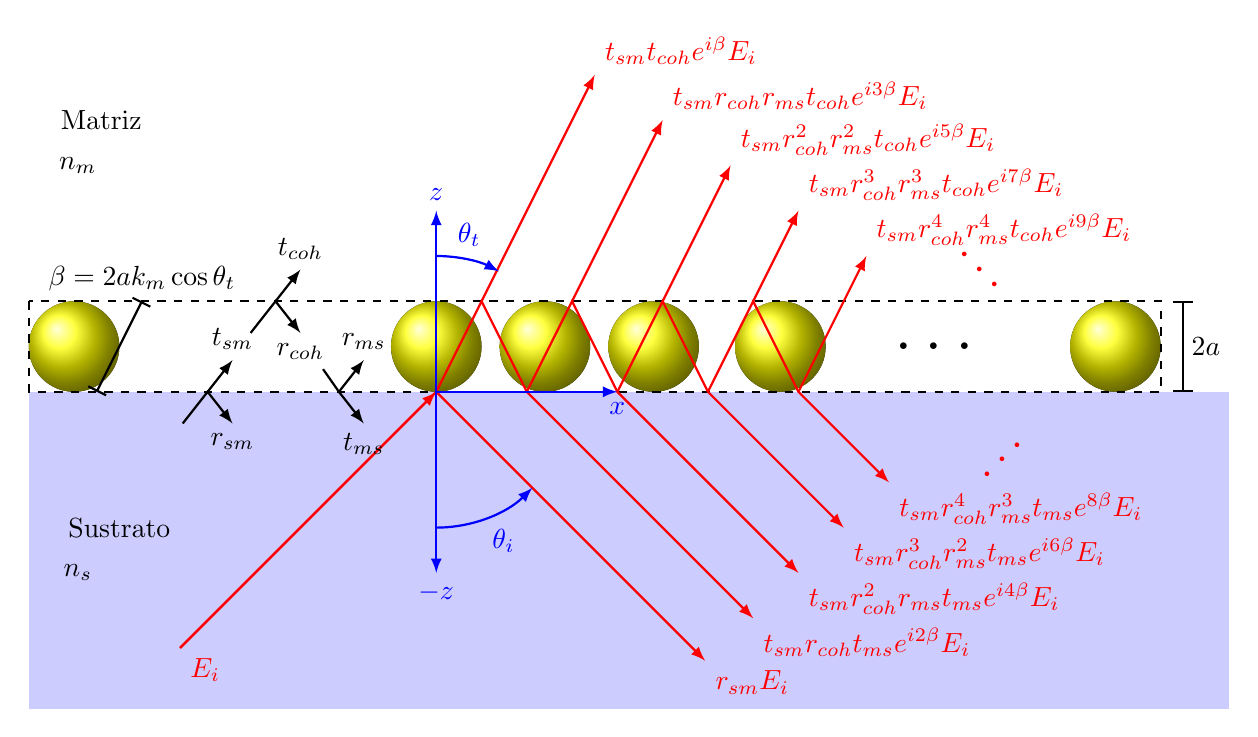
\begin{tikzpicture}[scale=1.15]
\def\a{.5}
\def\d{.5}
\def\t{.3}

\fill[blue, opacity = .2] (-4.5,-3.5) rectangle(8.75,0);

\foreach \x in {-4,0,1.2,2.4,3.8,7.5}{ %-2.9,-1.1
\fill[ball color=yellow, opacity=1] (\x,\d) circle(\a);}

\draw[thick, dashed] (-4.5,2*\d) rectangle (8,0);
\node at (5.5,\d) {\Huge $\ldots$};


%%%%%%%%%%%%%-------------Reflexiones
%
%\draw[latex -, thick, red](-135:0)--(-135:4) node[anchor=north]{$E_i$};
%\draw[- latex, thick, red](-135:4)--(-135:0)--(-45:4) node[anchor=north]{$r_{coh}E_i$};
%\draw[- latex, thick, red](0,0)--(2*\d,2*\d)--(3+2*\d,-3+2*\d) node[anchor=south west]{$t_{coh}r_{ms}t_{coh}E_i$};
%\draw[- latex, thick, red](4*\d,0)--(6*\d,2*\d)--(3+6*\d,-3+2*\d) node[anchor=south west]{$r_{coh}E_i$};


\draw[latex -, thick, red](-135:0)--(-135:4) node[anchor=north west]{$E_i$};
\draw[- latex, thick, red](-135:4)--(-135:0)--(-45:4.2) node[anchor=north west]{$r_{sm}E_i$};
\draw[- latex, thick, red](0,0)--(1*\d,2*\d)--(2*\d,0)--(3+\d,-3+\d) node[anchor=north west]{$t_{sm}r_{coh}t_{ms}e^{i2\beta}E_i$};
\draw[- latex, thick, red](2*\d,0)--(3*\d,2*\d)--(4*\d,0)--(3+2*\d,-3+2*\d) node[anchor=north west]{$t_{sm}r_{coh}^2r_{ms}t_{ms}e^{i4\beta}E_i$};
\draw[- latex, thick, red](4*\d,0)--(5*\d,2*\d)--(6*\d,0)--(3+3*\d,-3+3*\d) node[anchor=north west]{$t_{sm}r_{coh}^3r_{ms}^2t_{ms}e^{i6\beta}E_i$};
\draw[- latex, thick, red](6*\d,0)--(7*\d,2*\d)--(8*\d,0)--(3+4*\d,-3+4*\d) node[anchor=north west]{$t_{sm}r_{coh}^4r_{ms}^3t_{ms}e^{8\beta}E_i$};
\draw[-, thick, red](8*\d,0)--(9*\d,2*\d);
\node[rotate={45}] at (6.25,-.75) {\color{red}\LARGE $\ldots$};

%%%%%%%%%%%%%-------------transmisiones
\draw[- latex, thick, red](1*\d,2*\d)--(1.75,3.5) node[anchor=south west]{$t_{sm}t_{coh}e^{i\beta}E_i$};
\draw[- latex, thick, red](3*\d,2*\d)--(2+1*\d,4-2*\d) node[anchor=south west]{$t_{sm}r_{coh}r_{ms}t_{coh}e^{i3\beta}E_i$};
\draw[- latex, thick, red](5*\d,2*\d)--(2+2.5*\d,4-3*\d) node[anchor=south west]{$t_{sm}r_{coh}^2r_{ms}^2t_{coh}e^{i5\beta}E_i$};
\draw[- latex, thick, red](7*\d,2*\d)--(2+4*\d,4-4*\d) node[anchor=south west]{$t_{sm}r_{coh}^3r_{ms}^3t_{coh}e^{i7\beta}E_i$};
\draw[- latex, thick, red](9*\d,2*\d)--(2+5.5*\d,4-5*\d) node[anchor=south west]{$t_{sm}r_{coh}^4r_{ms}^4t_{coh}e^{i9\beta}E_i$};
\node[rotate={-45}] at (6,1.35) {\color{red}\LARGE $\ldots$};



\node at (-4,2.5) {$\; n_m$};
\node at (-3.7,3) {Matriz};
\node at (-4,-2) {$\; n_s$};
\node at (-3.5,-1.5) {Sustrato};

%\draw[latex - , thick](-2.8,-.5)--(-3.5,.5) node[anchor=north]{$r_{sm},\,t_{sm}$};
\draw[latex - , thick, shift ={(.55,0)}](-2.8,-.35)node[anchor=north]{$r_{sm}$}--(-3.075,0)--(-3.35,-.35);
\draw[latex -,thick, shift ={(.55,0)}](-2.8,.35)node[anchor=south]{$t_{sm}$}--(-3.075,0);
\draw[latex - , thick, shift ={(2.0,0)}](-2.8,-.35)node[anchor=north]{$t_{ms}$}--(-3.075,0)--(-3.25,.25);
\draw[latex -,thick, shift ={(2.0,0)}](-2.8,.35)node[anchor=south]{$r_{ms}$}--(-3.075,0);
\draw[latex - , thick, shift ={(1.3,2*\d)}](-2.8,-.35)node[anchor=north]{$r_{coh}$}--(-3.075,0)--(-3.35,-.35);
\draw[latex -,thick, shift ={(1.3,2*\d)}](-2.8,.35)node[anchor=south]{$t_{coh}$}--(-3.075,0);

\draw[|-|,thick, shift ={(-3.75,0)}](0,0)--(1*\d,2*\d) node[anchor=south]{$\beta = 2ak_m\cos\theta_t$};

\draw[|-|,thick, shift ={(8.25,0)}](0,0)--(0,2*\d) ;
\node at (8.5,\d){$2a$};

\draw[- latex, thick, blue] (0,0)--(90:2) node[anchor = south]{$z$};
\draw[- latex, thick, blue] (0,0)--(90:-2) node[anchor = north]{$-z$};
\draw[- latex, thick, blue] (0,0)--(0:2) node[anchor = north]{$x$};
\path (0,0)++(85:1.5)node[anchor=south west, blue]{$\theta_t$}; 
\draw[- latex, thick, blue](90:1.5)arc(90:62.5:1.5);
\path (0,0)++(-70:1.5)node[anchor=north west, blue]{$\theta_i$}; 
\draw[- latex, thick, blue](-90:1.5)arc(-90:-45:1.5);


\end{tikzpicture}
	\caption{ Esquema de las múltiples reflexiones en ATR del sistema matriz-monocapa-sustrato producidos por una onda plana $\vb{E}^i$ que incide en la interfaz de un sustrato, con índice de refracción $n_s$, que sostiene a una monocapa de NPs esféricas de radio $a$ inmersa en una matriz con $n_m$, a un ángulo $\theta_i$ respecto a la dirección normal a la interfaz. Las reflexiones y transmisiones en la interfaz sustrato-matriz ($z=0$) se describen por los coeficientes de amplitud de Fresnel [Ecs. \eqref{eq:rs}--\eqref{eq:tp}] en $\theta_i$, mientras que en la intfaz monocapa-matriz ($z=2a$) las reflexiones y transmisiones son descritas por el CSM [Ecs. \eqref{eqs:rtcoh}] en $\theta_t$. En los coeficientes de amplitud  $r_{\alpha\beta}$ y $t_{\alpha\beta}$ el medio de incidencia del haz de luz es $\alpha$ y el de transmisión en $\beta$.}\label{fig:CSM-ATR}
	\end{figure}



	\begin{align}
	r =& r_{sm} + t_{sm}r_{coh}t_{ms}e^{2i\beta}\left[1+r_{coh}r_{ms}e^{2i\beta}+\qty(r_{coh}r_{ms}e^{2i\beta})^2+\qty(r_{coh}r_{ms}e^{2i\beta})^3+\ldots,\right] \notag \\
		=& r_{sm} + \frac{ t_{sm}r_{coh}t_{ms}e^{2i\beta}}
				{1-r_{ms}r_{coh}e^{i2\beta}}, \label{eq:r_ATR_preStokes} \\
	t =& t_{coh}t_{ms}e^{i\beta} \left[1+r_{coh}r_{ms}e^{2i\beta}+\qty(r_{coh}r_{ms}e^{2i\beta})^2+\qty(r_{coh}r_{ms}e^{2i\beta})^3+\ldots\right]
	=\frac{  t_{coh}t_{ms}e^{i\beta} }
				{1-r_{ms}r_{coh}e^{i2\beta}}.\notag
	\end{align}
%
Es posible reescribir la Ec. \eqref{eq:r_ATR_preStokes} empleando las relaciones de Stokes\footnote{Las relaciones de Stokes\index{Fresnel!coeficientes de amplitud de ($r,t$)!relaciones de Stokes} se deducen a partir de la invariancia de las ecuaciones de Maxwell ante inversiones temporales ($t\to -t$), y relacionan a los coeficientes de amplitud $r$ y $t$ evaluados en $\theta_i$ y $\theta_t$ para una interfaz entre medios no absorbentes. Las relaciones de Stokes son \cite{hecht1998optics,garcia2012multiple} $r_{it}(\theta_i) = -r_{ti}(\theta_t)$, $t_{it}(\theta_i) = 1+r_{it}(\theta_i)$, y $t_{ti}(\theta_t) = 1+r_{it}(\theta_t)$.}, por lo que se obtiene\index{Esparcimiento!Coherente, Modelo de (CSM)!coeficientes de amplitud!incidencia interna} \begin{subequations}\vspace*{-.75em}
%
\begin{tcolorbox}[title = Coeficientes de amplitud de CSM en configuración ATR, breakable ]
	\eqhalf{r = \frac{r_{sm}(\theta_i)+r_{coh}(\theta_t)e^{i2\beta}}
					{1-r_{coh}(\theta_t)r_{sm}(\theta_i)e^{2i\beta}},
	\label{seq:rCSMATR}}
	\eqhalf{t = \frac{t_{sm}(\theta_i)t_{coh}(\theta_t)e^{i\beta}}
									{1-r_{coh}(\theta_t)r_{ms}(\theta_t)e^{2i\beta}},
	\label{seq:tCSMATR}}
	
	con $\beta = 2a k_0n_m\cos\theta_t$.
	\end{tcolorbox}\label{eqs:rtCSMATR}\end{subequations}\vspace*{-.75em}





